%==============================================================================
% tento soubor pouzijte jako zaklad
% this file should be used as a base for the thesis
% Autoři / Authors: 2008 Michal Bidlo, 2019 Jaroslav Dytrych
% Kontakt pro dotazy a připomínky: sablona@fit.vutbr.cz
% Contact for questions and comments: sablona@fit.vutbr.cz
%==============================================================================
% kodovani: UTF-8 (zmena prikazem iconv, recode nebo cstocs)
% encoding: UTF-8 (you can change it by command iconv, recode or cstocs)
%------------------------------------------------------------------------------
% zpracování / processing: make, make pdf, make clean
%==============================================================================
% Soubory, které je nutné upravit nebo smazat: / Files which have to be edited or deleted:
%   projekt-20-literatura-bibliography.bib - literatura / bibliography
%   projekt-01-kapitoly-chapters.tex - obsah práce / the thesis content
%   projekt-01-kapitoly-chapters-en.tex - obsah práce v angličtině / the thesis content in English
%   projekt-30-prilohy-appendices.tex - přílohy / appendices
%   projekt-30-prilohy-appendices-en.tex - přílohy v angličtině / appendices in English
%==============================================================================
\documentclass[]{fitthesis} % bez zadání - pro začátek práce, aby nebyl problém s překladem
%\documentclass[english]{fitthesis} % without assignment - for the work start to avoid compilation problem
%\documentclass[zadani]{fitthesis} % odevzdani do wisu a/nebo tisk s barevnými odkazy - odkazy jsou barevné
%\documentclass[english,zadani]{fitthesis} % for submission to the IS FIT and/or print with color links - links are color
%\documentclass[zadani,print]{fitthesis} % pro černobílý tisk - odkazy jsou černé
%\documentclass[english,zadani,print]{fitthesis} % for the black and white print - links are black
%\documentclass[zadani,cprint]{fitthesis} % pro barevný tisk - odkazy jsou černé, znak VUT barevný
%\documentclass[english,zadani,cprint]{fitthesis} % for the print - links are black, logo is color
% * Je-li práce psaná v anglickém jazyce, je zapotřebí u třídy použít 
%   parametr english následovně:
%   If thesis is written in English, it is necessary to use 
%   parameter english as follows:
%      \documentclass[english]{fitthesis}
% * Je-li práce psaná ve slovenském jazyce, je zapotřebí u třídy použít 
%   parametr slovak následovně:
%   If the work is written in the Slovak language, it is necessary 
%   to use parameter slovak as follows:
%      \documentclass[slovak]{fitthesis}
% * Je-li práce psaná v anglickém jazyce se slovenským abstraktem apod., 
%   je zapotřebí u třídy použít parametry english a enslovak následovně:
%   If the work is written in English with the Slovak abstract, etc., 
%   it is necessary to use parameters english and enslovak as follows:
%      \documentclass[english,enslovak]{fitthesis}

% Základní balíčky jsou dole v souboru šablony fitthesis.cls
% Basic packages are at the bottom of template file fitthesis.cls
% zde můžeme vložit vlastní balíčky / you can place own packages here

% Kompilace po částech (rychlejší, ale v náhledu nemusí být vše aktuální)
% Compilation piecewise (faster, but not all parts in preview will be up-to-date)
% \usepackage{subfiles}
\usepackage{graphicx}
\usepackage{gensymb}
% Nastavení cesty k obrázkům
% Setting of a path to the pictures
%\graphicspath{{obrazky-figures/}{./obrazky-figures/}}
%\graphicspath{{obrazky-figures/}{../obrazky-figures/}}

%---rm---------------
\renewcommand{\rmdefault}{lmr}%zavede Latin Modern Roman jako rm / set Latin Modern Roman as rm
%---sf---------------
\renewcommand{\sfdefault}{qhv}%zavede TeX Gyre Heros jako sf
%---tt------------
\renewcommand{\ttdefault}{lmtt}% zavede Latin Modern tt jako tt

% vypne funkci šablony, která automaticky nahrazuje uvozovky,
% aby nebyly prováděny nevhodné náhrady v popisech API apod.
% disables function of the template which replaces quotation marks
% to avoid unnecessary replacements in the API descriptions etc.
\csdoublequotesoff



\usepackage{url}


% =======================================================================
% balíček "hyperref" vytváří klikací odkazy v pdf, pokud tedy použijeme pdflatex
% problém je, že balíček hyperref musí být uveden jako poslední, takže nemůže
% být v šabloně
% "hyperref" package create clickable links in pdf if you are using pdflatex.
% Problem is that this package have to be introduced as the last one so it 
% can not be placed in the template file.
\ifWis
\ifx\pdfoutput\undefined % nejedeme pod pdflatexem / we are not using pdflatex
\else
  \usepackage{color}
  \usepackage[unicode,colorlinks,hyperindex,plainpages=false,pdftex]{hyperref}
  \definecolor{hrcolor-ref}{RGB}{223,52,30}
  \definecolor{hrcolor-cite}{HTML}{2F8F00}
  \definecolor{hrcolor-urls}{HTML}{092EAB}
  \hypersetup{
	linkcolor=hrcolor-ref,
	citecolor=hrcolor-cite,
	filecolor=magenta,
	urlcolor=hrcolor-urls
  }
  \def\pdfBorderAttrs{/Border [0 0 0] }  % bez okrajů kolem odkazů / without margins around links
  \pdfcompresslevel=9
\fi
\else % pro tisk budou odkazy, na které se dá klikat, černé / for the print clickable links will be black
\ifx\pdfoutput\undefined % nejedeme pod pdflatexem / we are not using pdflatex
\else
  \usepackage{color}
  \usepackage[unicode,colorlinks,hyperindex,plainpages=false,pdftex,urlcolor=black,linkcolor=black,citecolor=black]{hyperref}
  \definecolor{links}{rgb}{0,0,0}
  \definecolor{anchors}{rgb}{0,0,0}
  \def\AnchorColor{anchors}
  \def\LinkColor{links}
  \def\pdfBorderAttrs{/Border [0 0 0] } % bez okrajů kolem odkazů / without margins around links
  \pdfcompresslevel=9
\fi
\fi
% Řešení problému, kdy klikací odkazy na obrázky vedou za obrázek
% This solves the problems with links which leads after the picture
\usepackage[all]{hypcap}

% Informace o práci/projektu / Information about the thesis
%---------------------------------------------------------------------------
\projectinfo{
  %Prace / Thesis
  project={BP},            %typ práce BP/SP/DP/DR  / thesis type (SP = term project)
  year={2020},             % rok odevzdání / year of submission
  date=\today,             % datum odevzdání / submission date
  %Nazev prace / thesis title
  title.cs={Konstrukce pera se skrytými senzory},  % název práce v češtině či slovenštině (dle zadání) / thesis title in czech language (according to assignment)
  title.en={Pen Design with Hidden Sensors}, % název práce v angličtině / thesis title in english
  %title.length={14.5cm}, % nastavení délky bloku s titulkem pro úpravu zalomení řádku (lze definovat zde nebo níže) / setting the length of a block with a thesis title for adjusting a line break (can be defined here or below)
  %sectitle.length={14.5cm}, % nastavení délky bloku s druhým titulkem pro úpravu zalomení řádku (lze definovat zde nebo níže) / setting the length of a block with a second thesis title for adjusting a line break (can be defined here or below)
  %Autor / Author
  author.name={Jakub},   % jméno autora / author name
  author.surname={Senčák},   % příjmení autora / author surname 
  %author.title.p={Bc.}, % titul před jménem (nepovinné) / title before the name (optional)
  %author.title.a={Ph.D.}, % titul za jménem (nepovinné) / title after the name (optional)
  %Ustav / Department
  department={UITS}, % doplňte příslušnou zkratku dle ústavu na zadání: UPSY/UIFS/UITS/UPGM / fill in appropriate abbreviation of the department according to assignment: UPSY/UIFS/UITS/UPGM
  % Školitel / supervisor
  supervisor.name={Martin},   % jméno školitele / supervisor name 
  supervisor.surname={Sakin},   % příjmení školitele / supervisor surname
  supervisor.title.p={Ing.},   %titul před jménem (nepovinné) / title before the name (optional)
  supervisor.title.a={},    %titul za jménem (nepovinné) / title after the name (optional)
  % Klíčová slova / keywords
  keywords.cs={konštrukcia pera, falšovanie podpisu}, % klíčová slova v českém či slovenském jazyce / keywords in czech or slovak language
  keywords.en={pen construction, signature forgery}, % klíčová slova v anglickém jazyce / keywords in english
  %keywords.en={Here, individual keywords separated by commas will be written in English.},
  % Abstrakt / Abstract
  abstract.cs={}, % abstrakt v českém či slovenském jazyce / abstract in czech or slovak language
  abstract.en={}, % abstrakt v anglickém jazyce / abstract in english
  %abstract.en={An abstract of the work in English will be written in this paragraph.},
  % Prohlášení (u anglicky psané práce anglicky, u slovensky psané práce slovensky) / Declaration (for thesis in english should be in english)
  declaration={Prohlašuji, že jsem tuto bakalářskou práci vypracoval samostatně pod vedením pana Martina Sakina.
%Další informace mi poskytli
Uvedl jsem všechny literární prameny, publikace a další zdroje, ze kterých jsem čerpal.},
  %declaration={I hereby declare that this Bachelor's thesis was prepared as an original work by the author under the supervision of Mr. X
% The supplementary information was provided by Mr. Y
% I have listed all the literary sources, publications and other sources, which were used during the preparation of this thesis.},
  % Poděkování (nepovinné, nejlépe v jazyce práce) / Acknowledgement (optional, ideally in the language of the thesis)
  acknowledgment={Ďakujem svojmu vedúcemu Martinovi Sakinovi, za jeho prístup a ochotu pri vedení tejto práce.},
  %acknowledgment={Here it is possible to express thanks to the supervisor and to the people which provided professional help
%(external submitter, consultant, etc.).},
  % Rozšířený abstrakt (cca 3 normostrany) - lze definovat zde nebo níže / Extended abstract (approximately 3 standard pages) - can be defined here or below
  %extendedabstract={Do tohoto odstavce bude zapsán rozšířený výtah (abstrakt) práce v českém (slovenském) jazyce.},
  %faculty={FIT}, % FIT/FEKT/FSI/FA/FCH/FP/FAST/FAVU/USI/DEF
  faculty.cs={Fakulta informačních technologií}, % Fakulta v češtině - pro využití této položky výše zvolte fakultu DEF / Faculty in Czech - for use of this entry select DEF above
  faculty.en={Faculty of Information Technology}, % Fakulta v angličtině - pro využití této položky výše zvolte fakultu DEF / Faculty in English - for use of this entry select DEF above
  %department.cs={Ústav matematiky}, % Ústav v češtině - pro využití této položky výše zvolte ústav DEF nebo jej zakomentujte / Department in Czech - for use of this entry select DEF above or comment it out
  %department.en={Institute of Mathematics} % Ústav v angličtině - pro využití této položky výše zvolte ústav DEF nebo jej zakomentujte / Department in English - for use of this entry select DEF above or comment it out
}

% Rozšířený abstrakt (cca 3 normostrany) - lze definovat zde nebo výše / Extended abstract (approximately 3 standard pages) - can be defined here or above
%\extendedabstract{Do tohoasdto odstavce bude zapsán výtah (abstrakt) práce v českém (slovenském) jazyce.}

% nastavení délky bloku s titulkem pro úpravu zalomení řádku - lze definovat zde nebo výše / setting the length of a block with a thesis title for adjusting a line break - can be defined here or above
%\titlelength{14.5cm}
% nastavení délky bloku s druhým titulkem pro úpravu zalomení řádku - lze definovat zde nebo výše / setting the length of a block with a second thesis title for adjusting a line break - can be defined here or above
%\sectitlelength{14.5cm}

% řeší první/poslední řádek odstavce na předchozí/následující stránce
% solves first/last row of the paragraph on the previous/next page
\clubpenalty=10000
\widowpenalty=10000

% checklist
\newlist{checklist}{itemize}{1}
\setlist[checklist]{label=$\square$}

\begin{document}
  % Vysazeni titulnich stran / Typesetting of the title pages
  % ----------------------------------------------
  \maketitle
  % Obsah
  % ----------------------------------------------
  \setlength{\parskip}{0pt}

  {\hypersetup{hidelinks}\tableofcontents}
  
  % Seznam obrazku a tabulek (pokud prace obsahuje velke mnozstvi obrazku, tak se to hodi)
  % List of figures and list of tables (if the thesis contains a lot of pictures, it is good)
  \ifczech
    \renewcommand\listfigurename{Seznam obrázků}
  \fi
  \ifslovak
    \renewcommand\listfigurename{Zoznam obrázkov}
  \fi
  % {\hypersetup{hidelinks}\listoffigures}
  
  \ifczech
    \renewcommand\listtablename{Seznam tabulek}
  \fi
  \ifslovak
    \renewcommand\listtablename{Zoznam tabuliek}
  \fi
  % {\hypersetup{hidelinks}\listoftables}

  \ifODSAZ
    \setlength{\parskip}{0.5\bigskipamount}
  \else
    \setlength{\parskip}{0pt}
  \fi

  % vynechani stranky v oboustrannem rezimu
  % Skip the page in the two-sided mode
  \iftwoside
    \cleardoublepage
  \fi

  % Text prace / Thesis text
  % ----------------------------------------------
  % Tento soubor nahraďte vlastním souborem s obsahem práce.
%=========================================================================
% Autoři: Michal Bidlo, Bohuslav Křena, Jaroslav Dytrych, Petr Veigend a Adam Herout 2019
\chapter{Úvod}

TODO
°
\chapter{Teoretická část}

\section{Vlastnosti písania}

TODO
V tejto časti popíšem aké dáta chceme merať z písma.

\section{Existující technologie}

\subsection*{Livescribe 3}

Livescribe 3 je určené na písanie poznámok. Toto pero využíva Bluetooth v4.0 na spojenie s mobilným zariadením, do ktorého následne odosiela dáta o pohybe. Systém tieto dáta v reálnom čase prevádza do písaného textu, pričom je možné použiť aj funkciu konvertovania písaného textu do tlačenej podoby. Na záznam využíva infračervenú kameru, ktorá sa nachádza na spodnej časti pera pod hrotom tuhy. Okrem písma zaznamenáva aj zvuk a tak písmo doplňuje ďalší kontext. Veľkosťou je sa jedná o pomerne kompaktné zariadenie - 162x14.9 mm a hmotnosťou 34 gramov.\newline

\textbf{Hodnotenie:}
\begin{description}
	\item[+]{kompaktnosť}
	\item[+]{presnosť}
	\item[+]{nevyžaduje kalibráciu}
	\item[-]{infračervená kamera je príliš veľká, aby si ju používateľ nevšimol}
\end{description}

\subsection*{iskn Slate 2+}

Slate 2+ od firmy iskn využíva magnetický prstenec a špeciálnu podložku, v ktorej sa nachádza 32 magnetometrov (senzorov na meranie zmien magnetického poľa). Podložka komunikuje s aplikáciou v mobilnom zariadení alebo počítači pomocou Bluetooth LE 5.0 a v reálnom čase tieto dáta zobrazuje. Výsledok je veľmi presný, no vyžaduje presnú kalibráciu.\newline

\begin{figure}[hbt]
	\centering
	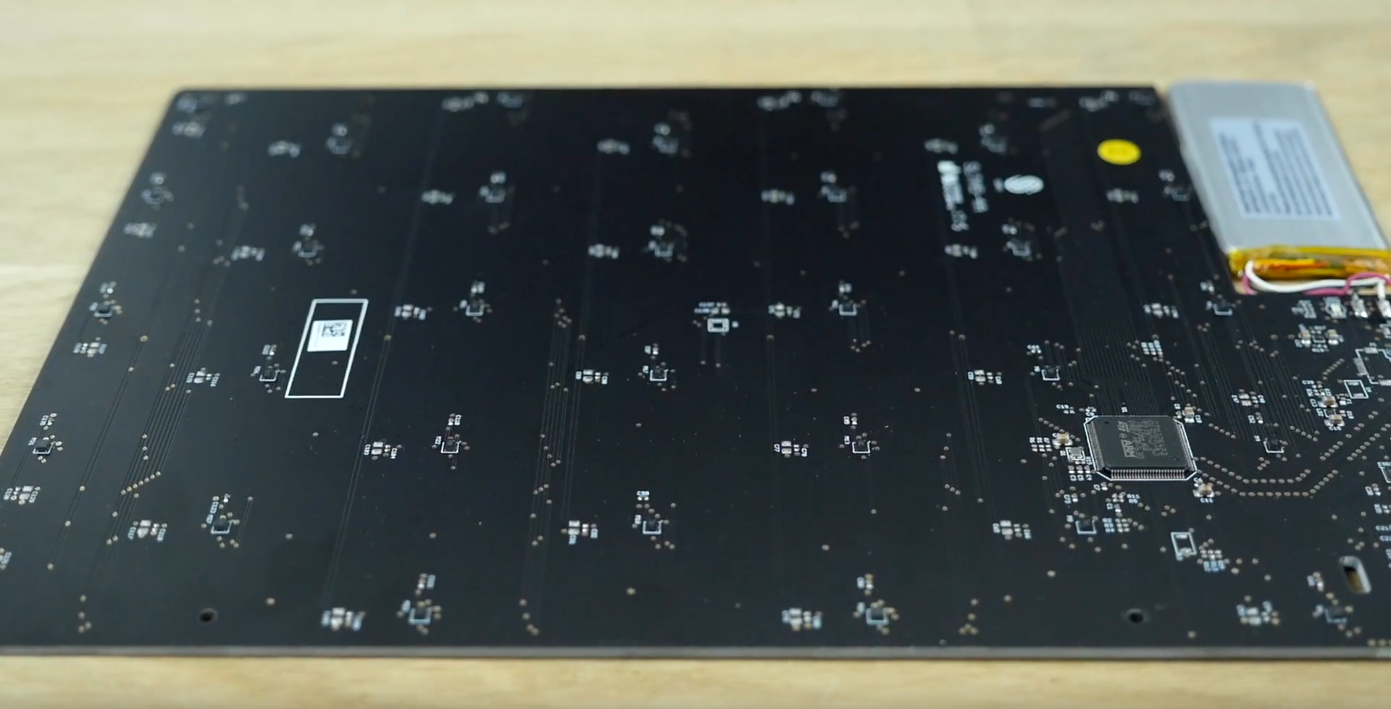
\includegraphics[width=0.5\textwidth]{obrazky-figures/isknBoard.png}
	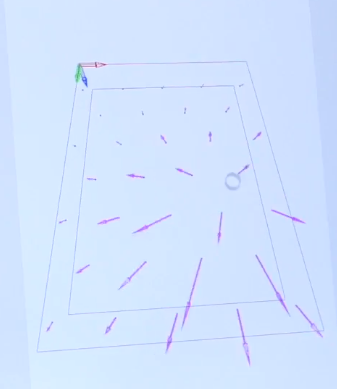
\includegraphics[width=0.3\textwidth]{obrazky-figures/isknMagneticfield.png}
	\caption{Board with sensors (left) and detected field (right)}
	\label{piezoPen1997}
\end{figure}
%isknMagneticfield
\textbf{Hodnotenie:}
\begin{description}
	\item[+]{nezáleží na použitom pere}
	\item[+]{písať sa môže čímkoľvek}
	\item[-]{vyžaduje podložku}
	\item[-]{kalibrácia}
\end{description}

\subsection*{Stylus}

Stylus sa používa na písanie na dotykové plochy. Aktuálne asi najsofistikovanejším je Apple Pencil. Radí sa mezdi aktívne stylusy\cite{HarleyJonahA2013As}. Používa dva trojosé gyroskopy rozmiestnené v rôznych častiach pera. Hrot pera funguje ako tlakový senzor a taktiež ako anténa, ktorá vysiela nízkofrekvenčné (dlhé) vlny a tie sú detekované senzorovou vrstvou pod displejom. Spojenie s iPadom zabezpečuje Bluetooth 4.1\cite{ApplePencilForum}. Intel v roku 2014 predpovedal, že aktívne stylusy nebudú také úspešné ako pasívne z dôvodu vysokej ceny a náročnosti vývoja takej technológie\cite{IntelDisp}. No ako môžeme vidieť, táto technológia nakoniec prerazila.\newline

\textbf{Hodnotenie:}
\begin{description}
	\item[+]{vysoká presnosť}
	\item[+]{realtime}
	\item[+]{nie je potrebná kalibrácia}
	\item[-]{náročnosť a komplexnosť vývoja}
	\item[-]{vyžaduje displej ako špeciálnu podložku}
	\item[-]{vysoká cena (keď rátame aj HW + displej a proprietárny software)}
	\item[-]{nefunguje so všetkými displejmi}
\end{description}

\subsection*{Návrh pera z roku 1977}

Jedná sa o pero so špeciálnou tuhou, ktorá má na sebe dva analógové piezoelektrické biomorfné senzory umiestnené v 90\degree~uhle k sebe navzájom. Podľa toho akou silou pôsobíme na hrot dokáže zaznamenať pohyb vďaka piezoeelktrickým javom.\cite{EernisseE}

\begin{figure}[hbt]
	\centering
	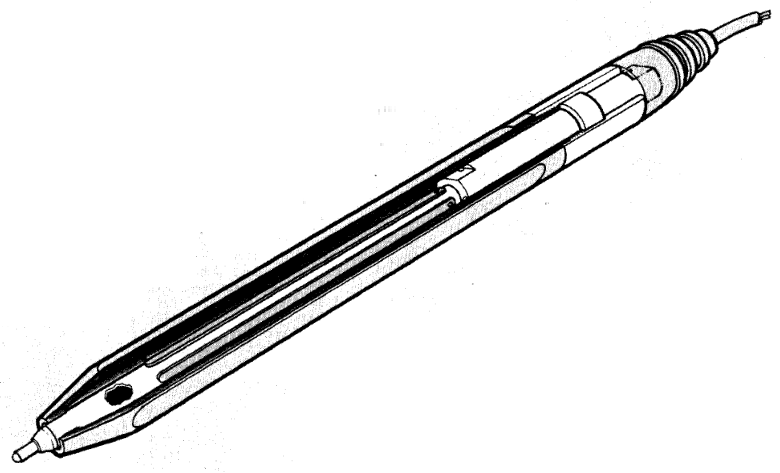
\includegraphics[width=0.3\textwidth]{obrazky-figures/piezoPen1997.png}
	\caption{Piezoelektrické pero}
	\label{piezoPen1997}
\end{figure}

\chapter{Návrh řešení}

V tejto časti sa budem venovať výberu komponent a samotnému návrhu pera so senzormi.

\section{Výber komponent}

\subsection*{Tlakový senzor}

Interlink Electronics FSR® 400 je malý a lacný tlakový odporový senzor. Bez záťaže sa správa ako nekonečný odpor a s použitím sily na jeho povrch sa jeho odpor znižuje. Citlivosť a maximálna záťaž je nastavená na interakciu s ľuďmi. \cite{fsr400}
V kombinácii s 10K Ohm rezistorom a zapojením na analógový pin dáva najširí interval hodnôt.

\subsection*{Akcelerometer a akcelerometer}

Rozhodol som sa použiť modul GY-521, ktorý kombinuje obidva senzory na jednom čipe. Akcelerometre typu MEMS trpia zvýšenou hladinou šumu\cite{PawlusJan2019Zpns}, ako som sa aj ja presvedčil. Zatiaľ som mal k dispozícii len jeden modul preto som zatiaľ neotestoval použitie dvoch modulov a priemerovanie nameraných hodnôt. Ako alternatívu teraz čakám na ďalšie dva senzory DFROBOT SEN0253\cite{PohybovySenzor}, na ktorých vyskúšam priemerovanie a rôzne rozmiestnenie na pere.

\subsection*{SD karta}

Výber padol na adaptér microSD kariet DFROBOT DFR0229 kvôli jeho veľkosti a jednoduchému pripojeniu. Ako úložisko používam MicroSD kartu veľkosti 2GB. 

\subsection*{Mikrokontrolér}

Na začiatku som si vybral vývojovú dosku Arduino Nano kvôli jej jednoduchému použitiu a programovaniu. 
Počiatočné experimenty však ukázaly, že táto doska nie je vhodná, pretože jej ADC (analógovo digitálny prevodník) je príliš pomalý pri spracovávaní z viacerých senzorov. Mikrokontrolér dokázal spracovať\footnote{prečítať aktuálnu hodnotu z výstupu a zapísať ju do pamäte FLASH na SD karte} len asi 100 hodnôt za sekundu, čo je v mojom prípade málo, keže jeden podpis trvá približne do dvoch sekúnd.

Teraz som začal hľadať iný mikrokontrolér a vyskúšam vývojovú dosku ARMSTM32F103C8T6 \cite{ArduinoARM}. Tiež budem kontaktovať pána Ing. Václava Šimeka, ktorý mi hádam poradí ďalej.


\section{Návrh pera}

\subsection*{Uchytenie tlakových senzorov}

\begin{figure}[hbt]
	\centering
	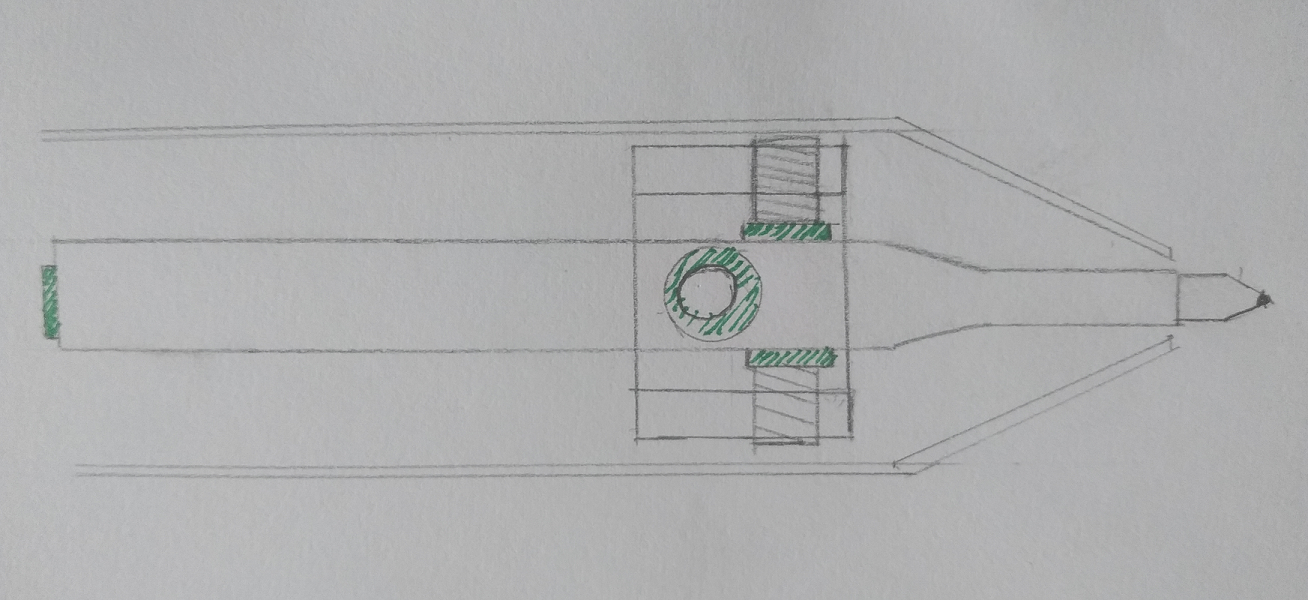
\includegraphics[width=1\textwidth]{obrazky-figures/umiestnenie_tlakovych_senzorov.png}
	\caption{Návrh uchytenia tuhy}
	\label{piezoPen1997}
\end{figure}

\begin{figure}[hbt]
	\centering
	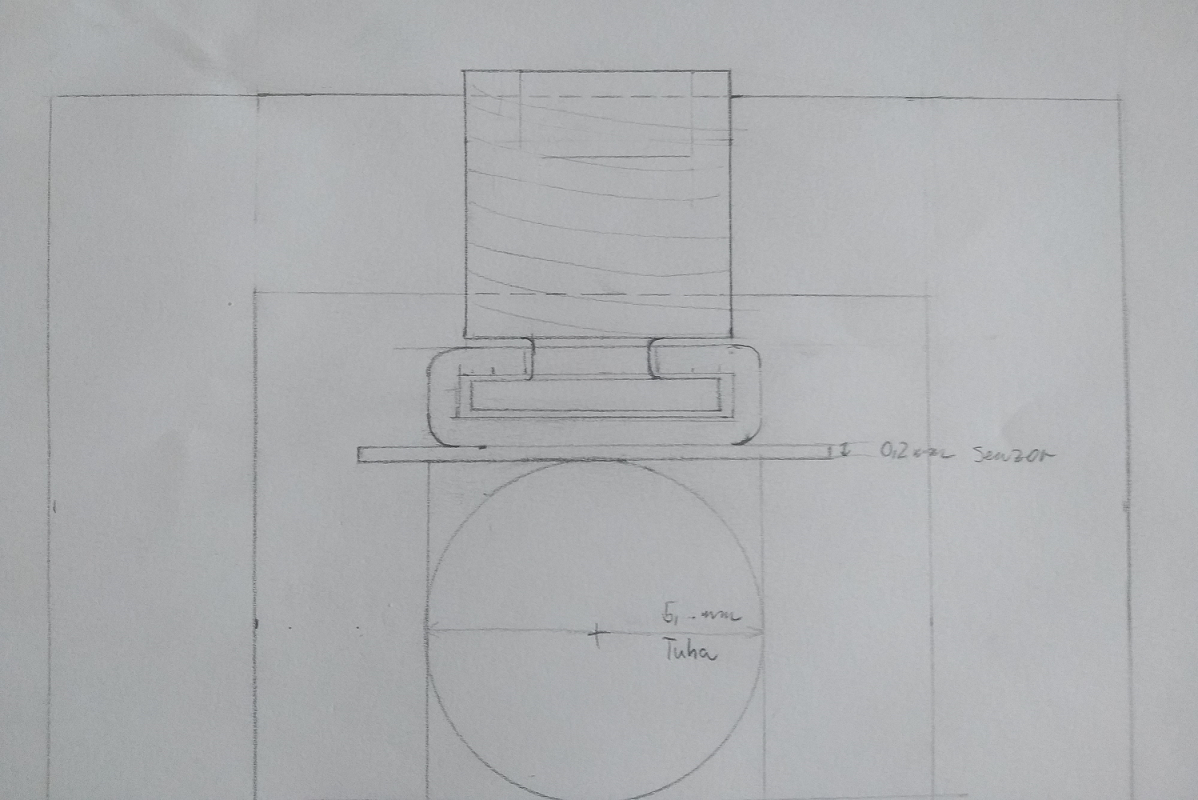
\includegraphics[width=1\textwidth]{obrazky-figures/uchytenie.png}
	\caption{Návrh uchytenia tlakového senzora}
	\label{piezoPen1997}
\end{figure}

\section{Nepoužité komponenty}

V tejto časti v skratke popíšem, ktoré súčiastky by sa mohli použiť v ďaľích prototypoch.

Mikrofón by sa mohol použiť ako senzor pre zachytenie širšieho kontextu, podobne ako to má Livescribe 3. Vedeli by sme potom k čomu sa písaný text viaže alebo aký dokument sa podpisuje. 

Ak by sme chceli merať ďalšie biometrické dáta mohli by sme použiť merač tepu na miestach kde sa človek dotýka pera. Ak bude osoba písať dlhší text vedeli by sme zistiť nakoľko je nervózna. 

Použitie bezdrôtového pripojenia, napr. BLE (Bluetooth Low Energy) by uľahčilo získavanie dát z pera, keďže ak sa chceme dostať k informáciám na SD karte musíme pero rozobrať. Toto riešnie by mohlo aj zmenšiť rozmery pera.

\chapter{Realizace řešení}

\section{Experimenty}

\subsection*{Testovanie súčiatok}

\begin{figure}[hbt]
	\centering
	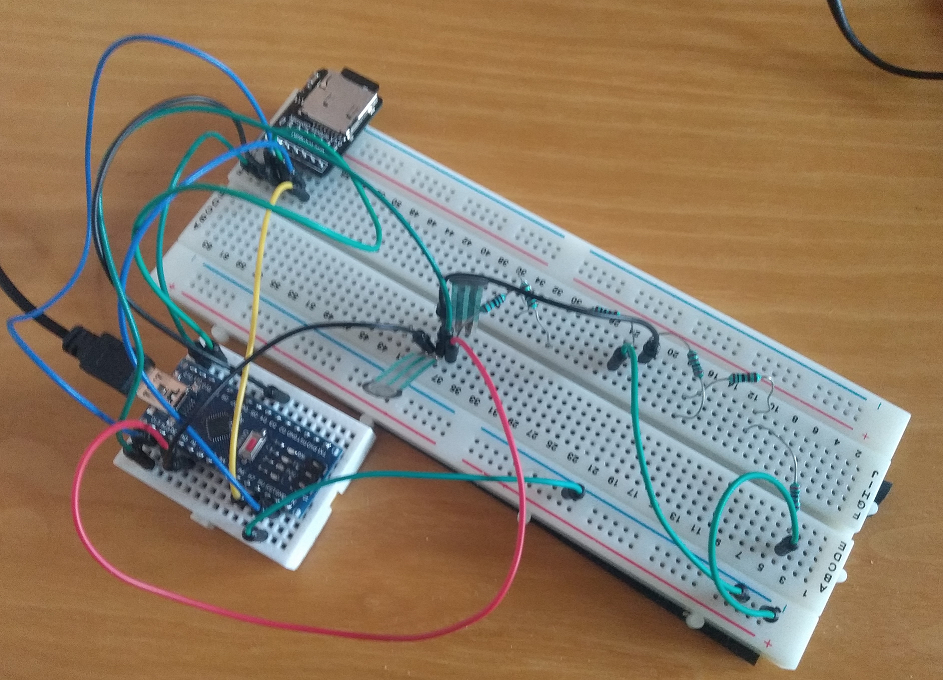
\includegraphics[width=0.5\textwidth]{obrazky-figures/FSRtestSD.png}
	\caption{Ukladanie dát na pamäťovú kartu}
	\label{Experiment1}
\end{figure}

\section{vyhodnocení výsledů}

\chapter{Závěr}

\label{zaver}

%===============================================================================

  
  
  % Kompilace po částech (viz výše, nutno odkomentovat)
  % Compilation piecewise (see above, it is necessary to uncomment it)
  %\subfile{projekt-01-uvod-introduction}
  % ...
  %\subfile{chapters/projekt-05-conclusion}


  % Pouzita literatura / Bibliography
  % ----------------------------------------------
\ifslovak
  \makeatletter
  \def\@openbib@code{\addcontentsline{toc}{chapter}{Literatúra}}
  \makeatother
  \bibliographystyle{bib-styles/Pysny/skplain}
\else
  \ifczech
    \makeatletter
    \def\@openbib@code{\addcontentsline{toc}{chapter}{Literatura}}
    \makeatother
    \bibliographystyle{bib-styles/Pysny/czplain}
  \else 
    \makeatletter
    \def\@openbib@code{\addcontentsline{toc}{chapter}{Bibliography}}
    \makeatother
    \bibliographystyle{bib-styles/Pysny/enplain}
  %  \bibliographystyle{alpha}
  \fi
\fi
  \begin{flushleft}
  \bibliography{literatura}
  \end{flushleft}

  % vynechani stranky v oboustrannem rezimu
  % Skip the page in the two-sided mode
  \iftwoside
    \cleardoublepage
  \fi

  % Prilohy / Appendices
  % ---------------------------------------------
  \appendix
\ifczech
  \renewcommand{\appendixpagename}{Přílohy}
  \renewcommand{\appendixtocname}{Přílohy}
  \renewcommand{\appendixname}{Příloha}
\fi
\ifslovak
  \renewcommand{\appendixpagename}{Prílohy}
  \renewcommand{\appendixtocname}{Prílohy}
  \renewcommand{\appendixname}{Príloha}
\fi
%  \appendixpage

% vynechani stranky v oboustrannem rezimu
% Skip the page in the two-sided mode
%\iftwoside
%  \cleardoublepage
%\fi
  
\ifslovak
%  \section*{Zoznam príloh}
%  \addcontentsline{toc}{section}{Zoznam príloh}
\else
  \ifczech
%    \section*{Seznam příloh}
%    \addcontentsline{toc}{section}{Seznam příloh}
  \else
%    \section*{List of Appendices}
%    \addcontentsline{toc}{section}{List of Appendices}
  \fi
\fi
  \startcontents[chapters]
  \setlength{\parskip}{0pt} 
  % seznam příloh / list of appendices
  % \printcontents[chapters]{l}{0}{\setcounter{tocdepth}{2}}
  
  \ifODSAZ
    \setlength{\parskip}{0.5\bigskipamount}
  \else
    \setlength{\parskip}{0pt}
  \fi
  
  % vynechani stranky v oboustrannem rezimu
  \iftwoside
    \cleardoublepage
  \fi
  
  % Přílohy / Appendices
  % Tento soubor nahraďte vlastním souborem s přílohami (nadpisy níže jsou pouze pro příklad)

% Umístění obsahu paměťového média do příloh je vhodné konzultovat s vedoucím
%\chapter{Obsah přiloženého paměťového média}

%\chapter{Manuál}

%\chapter{Konfigurační soubor}

%\chapter{RelaxNG Schéma konfiguračního souboru}

%\chapter{Plakát}

\chapter{Prílohy}

%--- Konec části převzaté z práce pana Pyšného ---
  
  
  % Kompilace po částech (viz výše, nutno odkomentovat)
  % Compilation piecewise (see above, it is necessary to uncomment it)
  %\subfile{projekt-30-prilohy-appendices}
  
\end{document}
